\chapter{Conceptional System Design}


\section{MVC Pattern}
\label{mvc}

The Model-View-Controller (MVC) is a software architecture pattern for user interface implementation, where the application logic is separated from the user interface.

In object-oriented programming the Model is the objects where the data from the database is stored. The View is the presentation layer, what the user sees and interacts with. The Controller will process and respond to the user requests and invoke the changes in the Model. 

The MVC pattern is memory efficient, because multiple views can share the same underlying data model. Controllers can be separated by events. This let's the developer to create a controller hierarchy, because a controller for a keyboard event is different from a controller for a mouse event. Views implement an instance of a controller, that can be changed at run-time, because we can be disabled and enabled.


\begin{figure}[!ht]
	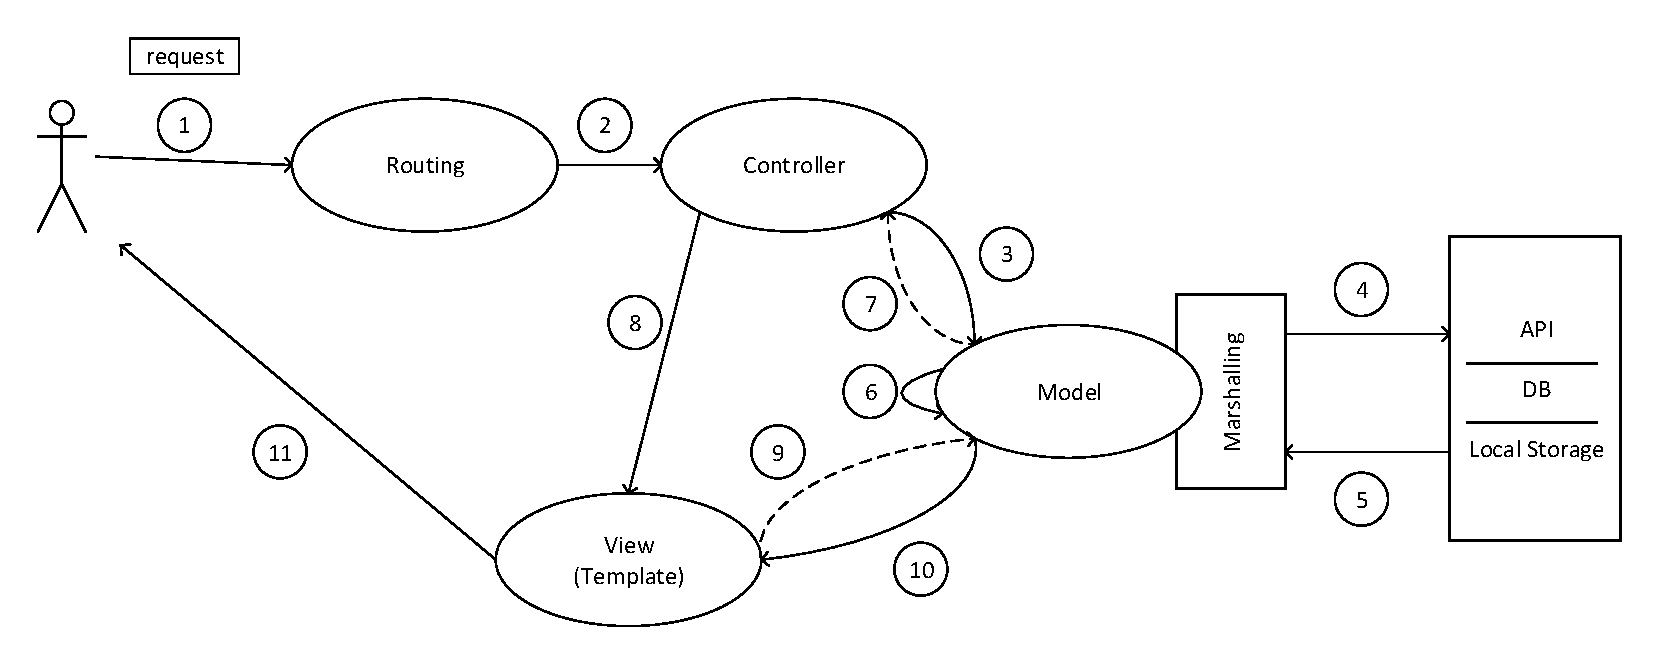
\includegraphics[width=\textwidth]{figures/klasszikus_mvc_webalkalmazas.pdf}
	\caption[Classic MVC Web Application]{Classic MVC Web Application\footnotemark}
	\label{fig:classic-mvc-webapplication}
\end{figure}
\footnotetext{Made by Bence Golda.}

In web applications the browser communicates with a controller. When the user sends a request, routing will decide which controller will handle the request. The chosen controller talks to the model to get the relevant data. If it's necessary, the model will send data to or ask for data from the database, the API or the local storage. During this process, the data has to be transformed via marshalling. Marshalling is the process, that transforms the data between storable and sendable dataformats. When the model returns the desired data to the controller, it will forward the data to the view. The presentation layer will decide which page has to be returned to the browser, binds the data to the view template and returns it.

\section{System Design}

\todo{bevezetőszöveg?}

\begin{figure}[!htbp]
	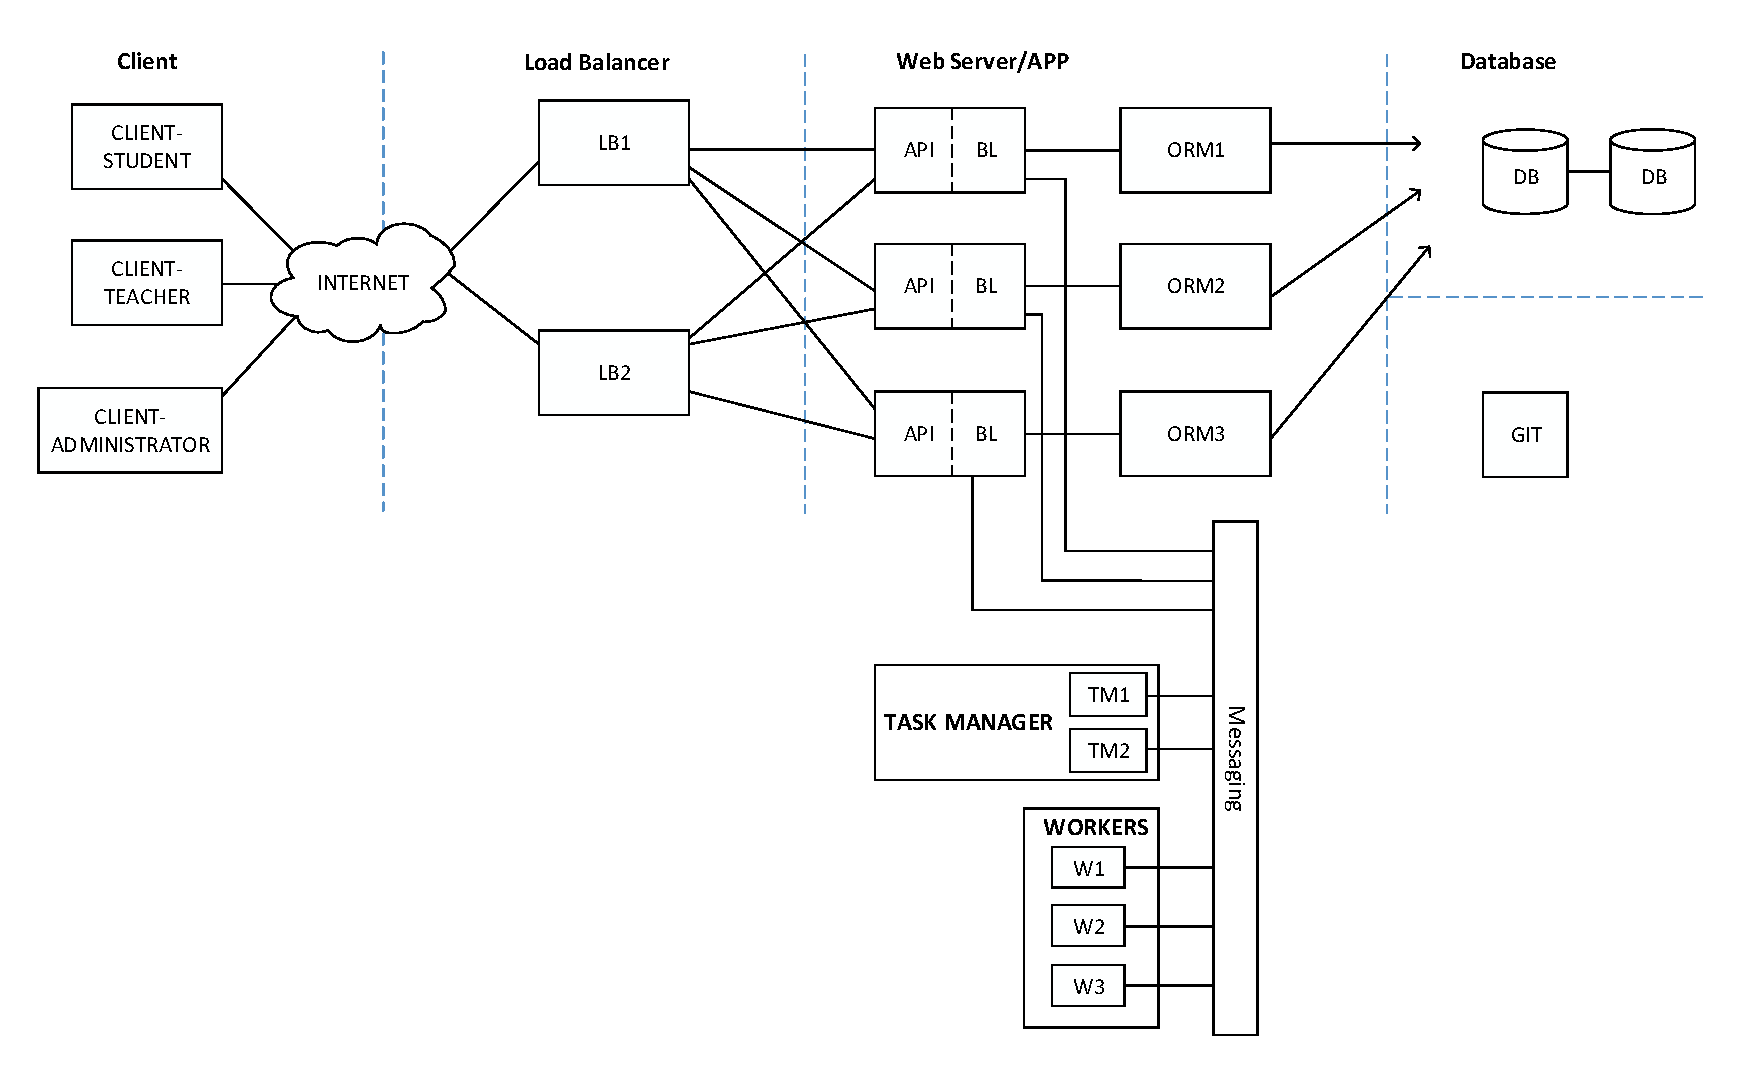
\includegraphics[width=0.95\textheight, angle=90]{figures/atfogo_rendszerterv_teljes.pdf}
	\caption[Conceptional System Design]{Conceptional System Design\\Made by the team.}
	\label{fig:conceptional-system-design}
\end{figure}

\todo{ábrán kijavítani, hogy a web server az külön szó}

The main components are the followings:

\begin{itemize}
	\item \textbf{Client:} A web portal, that is the communication bridge between the user and the web server. There will be three different modules: student, teacher and administrator. The different client modules can only communicate with the web server, and they cannot communicate with each other.
	\item \textbf{Database:} A database to store the system's data \see{ER-model}. 
	\item \textbf{Git:} A database to store the students' homeworks. Every student will get a different git repository for each laboratory.
	\item \textbf{Load Balancer:} It prevents the client from contacting the web server directly and solves the scalability problem. The client sends its requests to the load balancer, that will forward it to one of the web servers, depending on the client module, request type and the web servers' load.
	\item \textbf{Object-relational mapping:} It converts the data between the representation suitable for the implementation and the database. 
	\item \textbf{Message Bus:} A component, what supports messaging between the different components. The web server, the task manager, the message queue and the workers will use this to send tasks to each other.
	\item \textbf{Message Queue:} A component, what will forward the incoming tasks from the task manager to the right worker for processing. \todo{erről beszéljünk, hogy az MB miért nem elég nekünk}
	\item \textbf{Task Manager:} A special worker. It gets tasks from the web server to decide which worker has to process it. After the decision it forwards the task through the message bus.
	\item \textbf{Web Server:} The server that runs the API's implementation. This component processes the incoming requests, creates tasks and forwards them to the task manager. It also provides its clients the data from the databases. The API is written in Ruby on Rails. 
	\item \textbf{Worker:} This will process the task, e.g., changes the user's mailing list subscription.
\end{itemize}

\newpage
\subsubsection{Scalability}

\newparagraph{Client}

To solve the scalability problem, the client's code will run in a web browser for every user. This way, resources for the client's code are provided by the user as he opens the web portal in a web browser.
 
\newparagraph{Web Server}

If there were not any load balancer between the client and the web server, then one server would get every request. With thousands of users this could lead to overload and high the response time. With a load balancer, the requests will first arrive at the load balancer, and it will decide which web server will handle that request and forwards it to that web server. The choice depends on the client module, request type and the web servers' load. The load balancer's purpose is to avoid overload and minimize the response time.
 
\subsection{Frontend System Design}
\todo{frontend ábra visioban}

\subsection{Entity–relationship model}
\label{ER-model}

\begin{figure}[!htbp]
	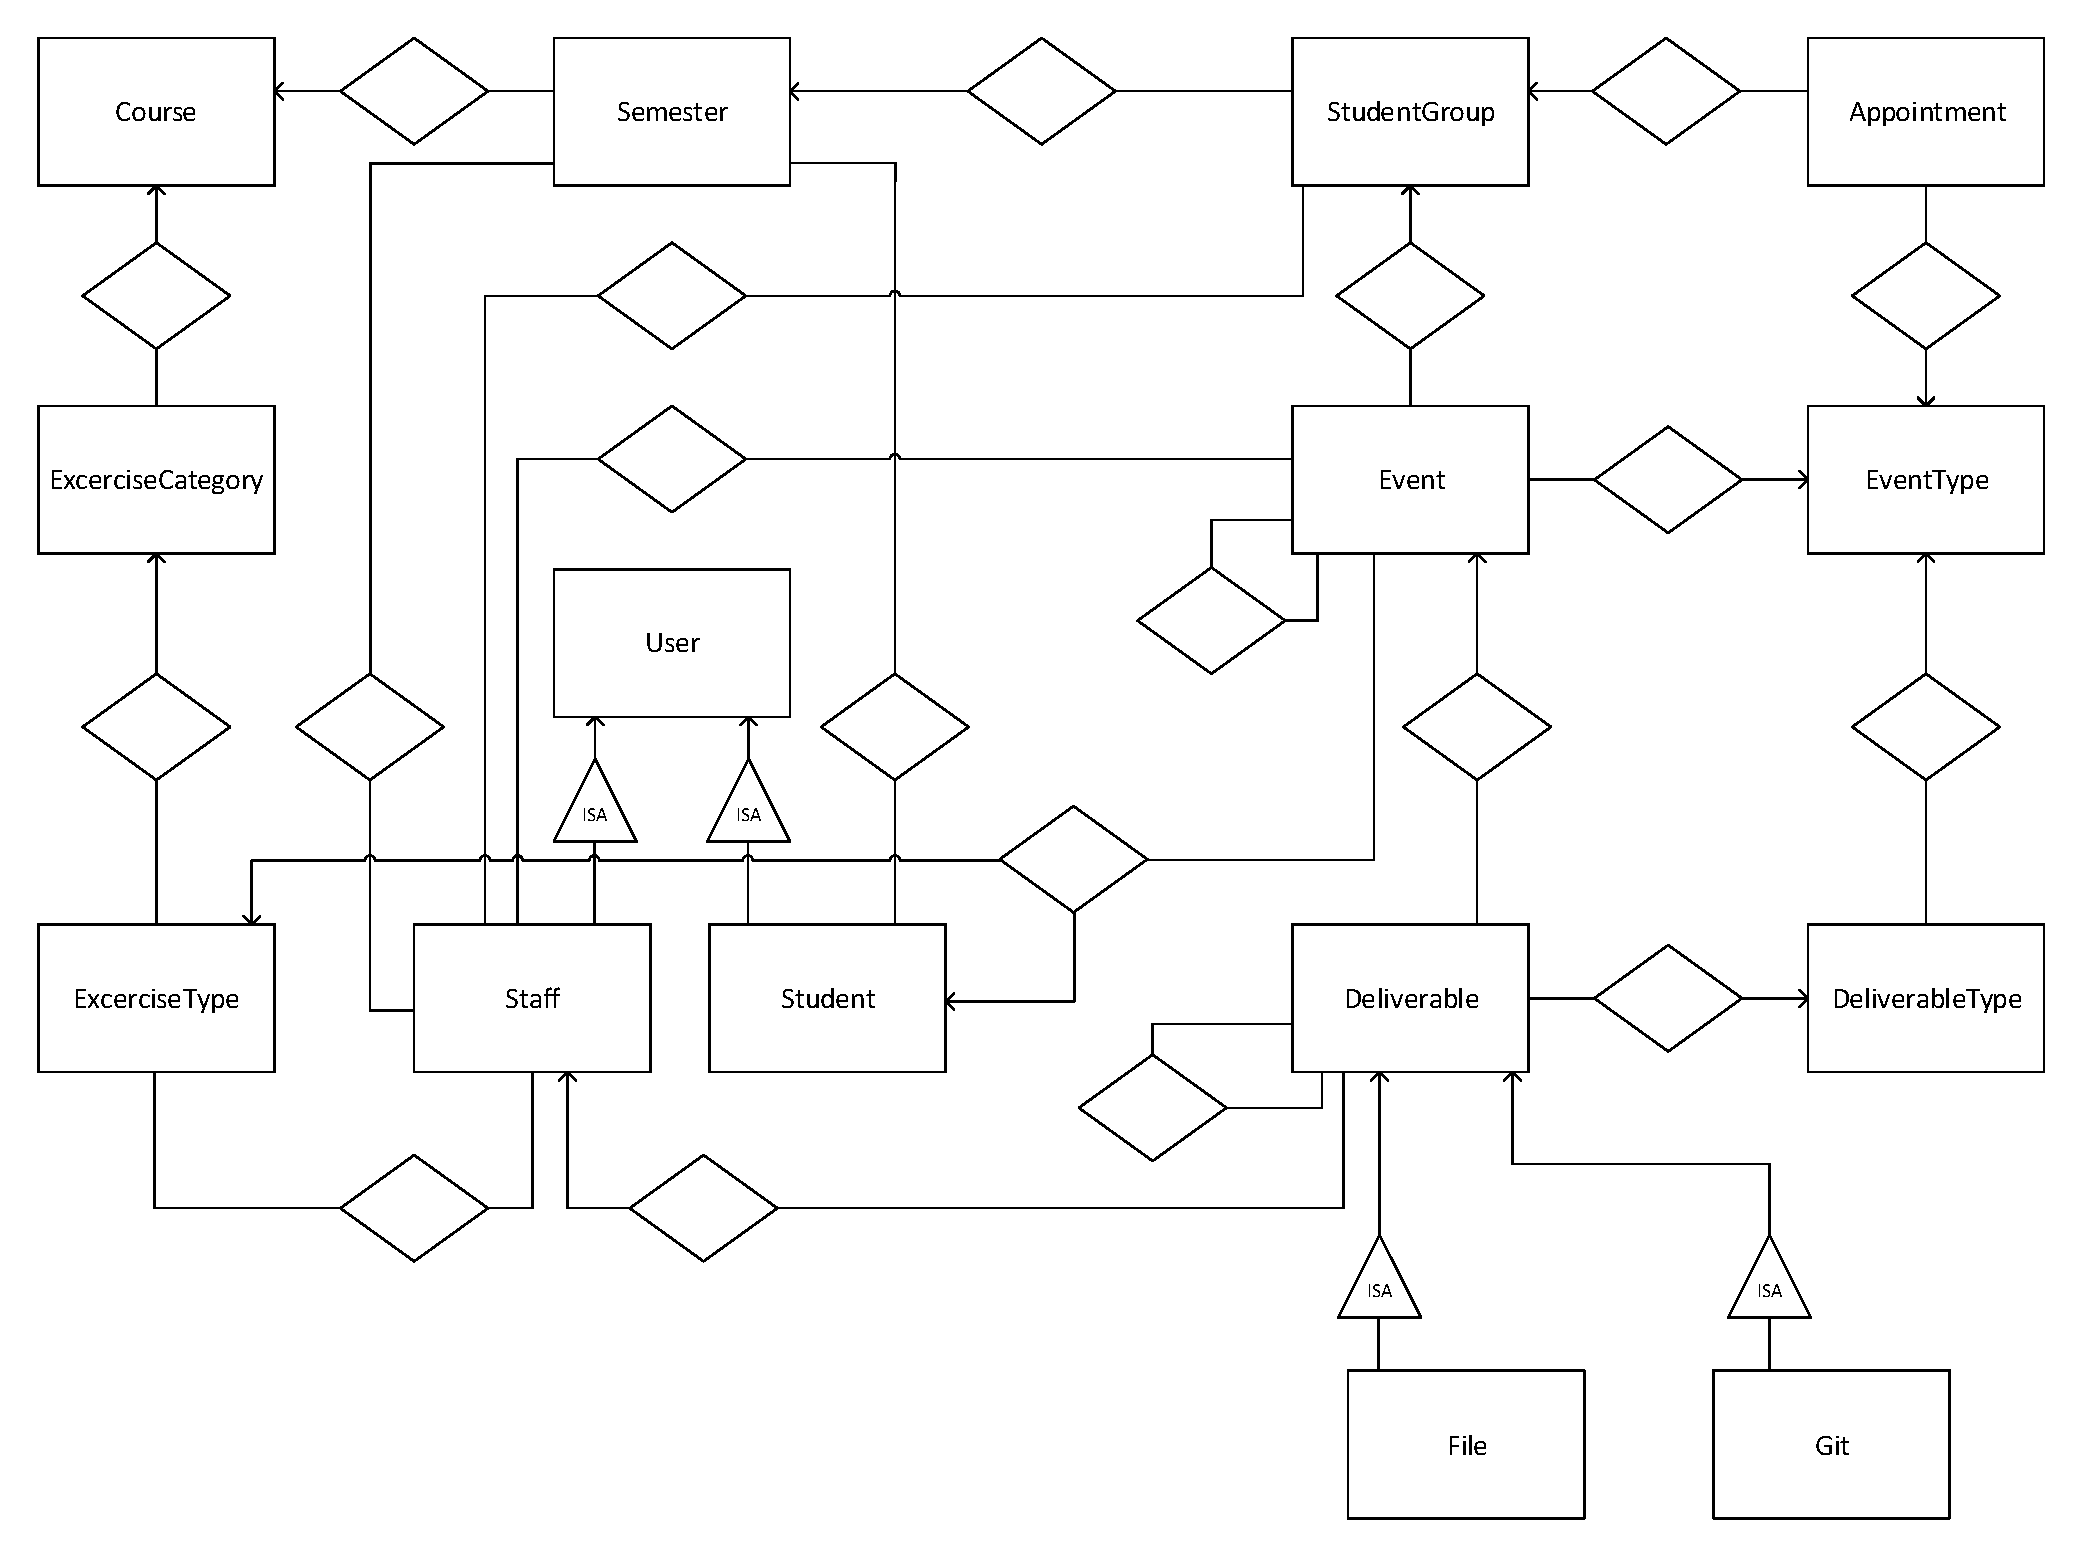
\includegraphics[width=0.85\textheight, angle=90]{figures/ER.pdf}
	\caption[Entity–relationship model]{Entity–relationship model\\Finalized by the team based on my proposal.}
	\label{fig:er}
\end{figure}


\todo{magyarázat}
